% !TEX TS-program = pdflatex
% !TEX encoding = UTF-8 Unicode

% This is a simple template for a LaTeX document using the "article" class.
% See "book", "report", "letter" for other types of document.

\documentclass[11pt]{article} % use larger type; default would be 10pt

\usepackage[utf8]{inputenc} % set input encoding (not needed with XeLaTeX)

%%% Examples of Article customizations
% These packages are optional, depending whether you want the features they provide.
% See the LaTeX Companion or other references for full information.

%%% PAGE DIMENSIONS
\usepackage{geometry} % to change the page dimensions
\geometry{a4paper} % or letterpaper (US) or a5paper or....
% \geometry{margin=2in} % for example, change the margins to 2 inches all round
% \geometry{landscape} % set up the page for landscape
%   read geometry.pdf for detailed page layout information

\usepackage{graphicx} % support the \includegraphics command and options

% \usepackage[parfill]{parskip} % Activate to begin paragraphs with an empty line rather than an indent

%%% PACKAGES
\usepackage{booktabs} % for much better looking tables
\usepackage{array} % for better arrays (eg matrices) in maths
\usepackage{paralist} % very flexible & customisable lists (eg. enumerate/itemize, etc.)
\usepackage{verbatim} % adds environment for commenting out blocks of text & for better verbatim
\usepackage{subfig} % make it possible to include more than one captioned figure/table in a single float
% These packages are all incorporated in the memoir class to one degree or another...

%%% HEADERS & FOOTERS
\usepackage{fancyhdr} % This should be set AFTER setting up the page geometry
\pagestyle{fancy} % options: empty , plain , fancy
\renewcommand{\headrulewidth}{0pt} % customise the layout...
\lhead{}\chead{}\rhead{}
\lfoot{}\cfoot{\thepage}\rfoot{}

%%% SECTION TITLE APPEARANCE
\usepackage{sectsty}
\allsectionsfont{\sffamily\mdseries\upshape} % (See the fntguide.pdf for font help)
% (This matches ConTeXt defaults)

%%% ToC (table of contents) APPEARANCE
\usepackage[nottoc,notlof,notlot]{tocbibind} % Put the bibliography in the ToC
\usepackage[titles,subfigure]{tocloft} % Alter the style of the Table of Contents
\renewcommand{\cftsecfont}{\rmfamily\mdseries\upshape}
\renewcommand{\cftsecpagefont}{\rmfamily\mdseries\upshape} % No bold!

%%% END Article customizations

%%% The "real" document content comes below...

\title{Lecture 15}
\author{TLS and secure channels}
%\date{} % Activate to display a given date or no date (if empty),
         % otherwise the current date is printed 

\begin{document}
\maketitle

\section{Common Crytographic Network Protocols}

\subsection{TLS (Transport Layer Security)}
\begin{itemize}
  \item  Used to provide an encryption wrapper around HTTP to make HTTPS, and for
  many other application layer protocols.
  \item TLS is wrapped around the application layer.
  \item Security goals: Authenticate server, confidentiality and integrity of
  traffic. Ensure that client is connected to the server they think they are
  connected to.
  \item Originally called the Secure Socket Layer (SSL).
\end{itemize}

\subsection{SSH (Secure Shell)}
\begin{itemize}
  \item Encrypted alternative to Telnet, Telnet uses an unencrypted connection
  that sends information in plaintext, which is easily exploitable.
  \item Security goals: Authenticate server and client, confidentiality and
  integrity of traffic.
\end{itemize}

\subsection{IPsec (Internet Protocol Security)}
\begin{itemize}
  \item Provides an encrypted, authenticated alternative to IP. Complicated set
  of protocols which attempt to replace the IP layer.
  \item Regular IP is insecure because anyone can view the payload of packets.
  \item Tunnel IPSec through IP.
  \item Commonly used for VPNs (Virtual Private Networks).
  \item Security goals: client and server authentication, authenticate headers,
  optionally encrypt headers, ensure confidentiality and integrity of payloads.
\end{itemize}

\section{Constructing a Secure Encrypted Channel}
\subsection{Encrypt and MAC data}
To construct a secure encrypted channel there are several steps of prelinary
communication that the client and server must perform before the channel can be
established.
\begin{center}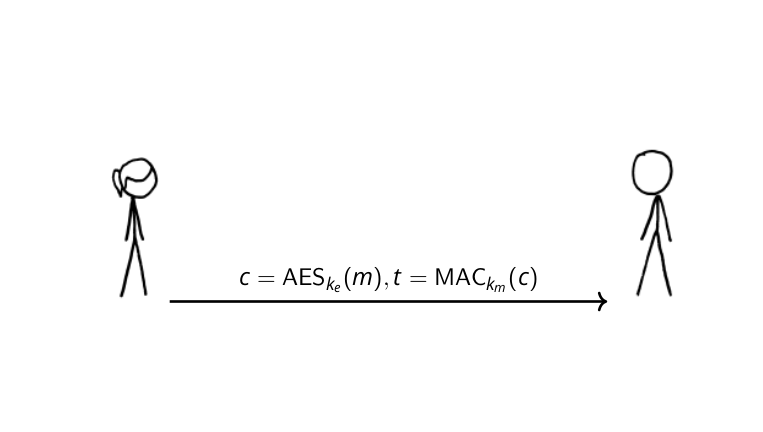
\includegraphics[scale=.8]{./tls1.png}\end{center}
Alice[left] and Bob[right] want to communicate on a secure channel on that is
protected against passive easedroppers and man-in-the-middle attacks. 

Assuming Alice and Bob have shared a set of keys, Alice sends her AES ciphertext
and the MAC of the ciphertext to Bob.  Bob can now check the MAC and decrypt the
cipher text to get the original message.

\subsection{Diffie-Hellman key exchange}
In order to negotiate and share encrypted MAC keys, there must be a
Diffie-Hellman key exchange.

\begin{center}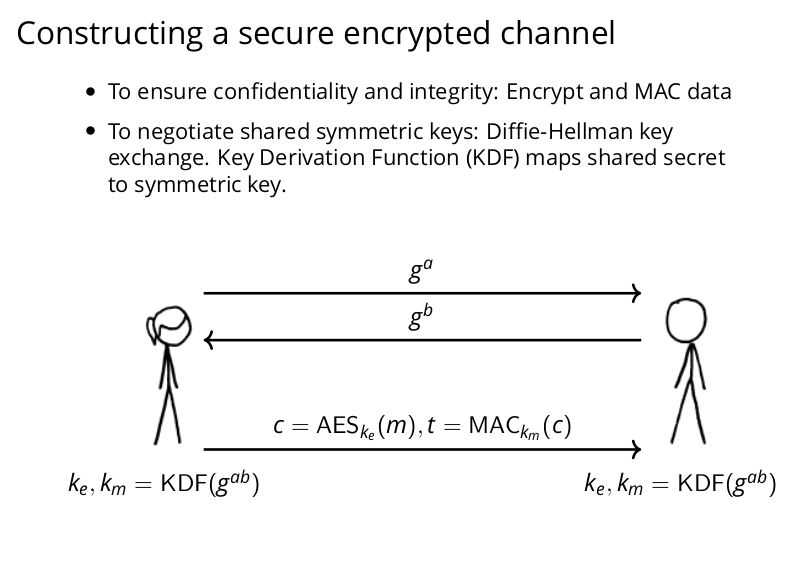
\includegraphics[scale=.8]{./tls2.png}\end{center}

\end{document}
